Les besoins fonctionnels sont ordonnés par ordre de priorité. En fonction de leur importance, ils sont notés de 1 à 3 (1 étant le niveau avec le plus de priorité). La priorité des besoins est déterminée par rapport à ce que nous jugeons être le plus important dans l'application. \\

Pour certains besoins, nous allons évoquer une machine de spécification minimale, c'est-à-dire, un ordinateur pouvant exécuter l'application avec des composants de puissance minimale. Une machine de spécification minimale doit donc être pourvue à minima de 4Go de mémoire vive, d'un simple processeur basique (ex : dual core 1.7Ghz), de 50Mo d'espace de stockage et ne nécessite pas de GPU.

\subsection{Besoins fonctionnels}

\subsubsection{Le lanceur de moteur de jeu}
\label{sec:launcher}

\begin{enumerate}

    \item \textbf{Analyser les arguments de la ligne de commande :}\\
    Pour connaître les paramètres de la partie, le programme du lanceur de moteur de jeu analyse les arguments et enregistre les valeurs données. Si le nom de l'argument n'est pas reconnu, il est ignoré (ainsi que sa valeur). Une valeur associée à un argument doit avoir une taille inférieure à 100 caractères. Si la valeur d'un argument n'est pas correct, le lanceur doit annoncer l'erreur et arrêter le logiciel. L'utilisateur, joueur ou non de la partie de jeu qui va suivre, décide de la valeur des arguments à fournir (ceci est alors valable et applicable pour les besoins qui suivent concernant les arguments de la ligne de commande). \\
    \textbf{Priorité :} 1. \\
    \textbf{Risques :}
    \begin{itemize}
        \item aucun argument n'est reconnu par le logiciel.
        \item un argument attend une valeur d'un type de donnée précis mais un autre est renseigné.
        \item un argument est trop long en nombre de caractères.
        \item un argument demandant une valeur, mais sans valeur spécifiée.
        \item un argument obligatoire n'est pas renseigné.
    \end{itemize}
    \textbf{Parade :} Afficher un message d'erreur, spécifiant le type d'erreur rencontré.
    
    \item \textbf{Sélectionner le type de joueur (humain/IA) :} \\
    L'argument \code{--joueurs} permet de donner le type ainsi que le nombre des joueurs participants. Les valeurs de ce paramètre peuvent être exprimées par ce regex \code{(<type> <nombre>? )+}. S'il n'y a pas de nombre fourni avec le type, la valeur par défaut, 1 (un), est choisie comme quantité. Une partie peut être lancée uniquement avec des joueurs IA, uniquement des joueurs humains ou les deux.
    Les types possibles sont \code{humain} (pour un joueur humain), \code{ia-basique} (pour une ia appliquant une stratégie basique), \code{ia-hilo} (pour une ia appliquant une stratégie Hi-Lo), \code{ia-hilo-nocount} (pour une ia appliquant une stratégie Hi-Lo sans méthode de comptage) et \code{ia-deep} (pour une ia utilisant le deeplearning). \\
    \textbf{Priorité :} 1. \\
    \textbf{Risques :}
    \begin{itemize}
        \item un type autre que \code{humain}, \code{ia-basique}, \code{ia-hilo}, \code{ia-hilo-nocount} ou \code{ia-deep} est donné.
        \item un nombre négatif est donné.
        \item le nombre total de joueur (humain + IA) est supérieur à 7.
    \end{itemize}
    \textbf{Parade :} Afficher un message d'erreur, spécifiant le type d'erreur rencontré.

    \item \textbf{Lancer un ensemble de parties de jeu :} \\
    Le paramètre \code{--parties <nombre>} permet de définir le nombre de parties que le logiciel va lancer. Le nombre de partie de Blackjack doit être compris entre 0 et 500 inclus.
    Un joueur n'a pas le droit de partir entre plusieurs parties (si le programme est lancé pour 10 parties, chaque joueur devra jouer les 10 parties). Dans le cas où cet argument n'est pas renseigné, le logiciel lancera une seule et unique partie, après laquelle le programme s'arrêtera. Les parties sont lancées consécutivement. Chaque partie se déroule selon les règles du blackjack et les valeurs des arguments passés dans la ligne de commande au départ. \\
    \textbf{Priorité :} 2. \\
    \textbf{Risques :}
    \begin{itemize}
        \item une valeur négative est donnée.
        \item une valeur supérieure à 500 est donnée.
    \end{itemize}
    \textbf{Parade :} Afficher un message d'erreur, spécifiant le type d'erreur rencontré.
    
    \item \textbf{Sélectionner la quantité d'argent de départ par joueur:}\\
    L'argument \code{--argent}, avec comme valeur une liste de nombre détermine la somme d'argent que les joueurs ont au départ de l'exécution. L'ordre de ces nombres correspond à l'ordre des joueurs déterminé par \code{--joueurs}.\\
    Par exemple \code{--joueurs humain 1 ia 2 --argent 10 20 10} se traduit par un joueur humain avec 10 dollars, un joueur IA avec 20 dollars et un joueur IA avec 10 dollars. La somme d'argent de départ d'un joueur doit être comprise entre 0 et 100 000 inclus. \\
    \textbf{Priorité :} 2. \\
    \textbf{Risques :}
    \begin{itemize}
        \item une valeur inférieure à 0 est donnée.
        \item une valeur supérieure à 100 000 est donnée.
        \item le nombre de valeur ne correspond pas au nombre de joueur.
    \end{itemize}
    \textbf{Parade :} Afficher un message d'erreur, spécifiant le type d'erreur rencontré.

    \item \textbf{Sélectionner le nombre de paquet de cartes à utiliser:}\\
    L'option \code{--paquets} détermine le nombre de paquet de cartes que le moteur utilisera durant le jeu. Le nombre de paquet doit être compris entre 1 et 7 inclus. Si il n'y a pas de nombre précisé, la valeur par défaut est 1. \\
    \textbf{Priorité :} 2. \\
    \textbf{Risques :}
    \begin{itemize}
        \item une valeur inférieure à 1 est donnée.
        \item une valeur supérieure à 7 est donnée.
    \end{itemize}
    \textbf{Parade :} Afficher un message d'erreur, spécifiant le type d'erreur rencontré.
    
    \vspace{1cm}
    \begin{figure}[H]
        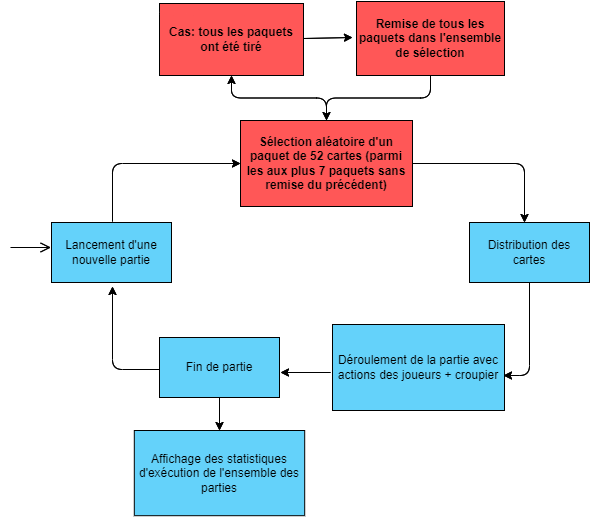
\includegraphics[width=\textwidth]{{2-besoins/diagramme_renouvellement_paquet.png}}
        \caption{Schéma d'utilisation et renouvellement de plusieurs paquets}
        \label{fig:diag_use_ren_deck}
    \end{figure}
    \vspace{0.5cm}
    
    \item \textbf{Afficher les statistiques d'exécution de l'ensemble des parties :} \\
    Après avoir lancé toutes les parties de Blackjack, le logiciel affiche les statistiques de ces parties de jeu (cf. \hyperref[itm:stats]{Afficher les statistiques liées à un ensemble de partie}). \\
    \textbf{Priorité :} 2. \\
    \textbf{Risques :} aucun. \\
    \textbf{Parade :} aucune.

    \item \textbf{Lire les paramètres du lanceur de moteur de jeu via un fichier:}\\
    Le fichier sera donné via l'argument \code{--fichier params.json}. Si cet argument existe, aucun autre argument n'est pris en compte dans la ligne de commande. C'est le fichier qui dicte les paramètres. Le format des données du fichier est JSON (cf. \nameref{sec:format}). \\
    \textbf{Priorité :} 3. \\
    \textbf{Risques :}
    \begin{itemize}
        \item le format du fichier ne correspond pas à un \code{.json}.
        \item le fichier est corrompu.
        \item les valeurs du fichier ne correspondent pas à des arguments.
        \item les arguments spécifiés ne sont pas complets.
    \end{itemize}
    \textbf{Parade :} Afficher un message d'erreur, spécifiant le type d'erreur rencontré.

    \item \textbf{Sélectionner la mise minimum:}\\
    L'argument \code{--mise-min} détermine la mise minimum par joueur. Cet argument est optionnel. Si il n'est pas renseigné, alors une mise minimum par défaut de 5 dollars est utilisée. La valeur de mise doit être comprise entre 5 et 100 000 inclus. \\
    \textbf{Priorité :} 3. \\
    \textbf{Risques :}
    \begin{itemize}
        \item une valeur inférieure à 5 est donnée.
        \item une valeur supérieure à 100 000 est donnée.
    \end{itemize}
    \textbf{Parade :} Afficher un message d'erreur, spécifiant le type d'erreur rencontré.
    
    \vspace{1cm}
    \begin{figure}[H]
        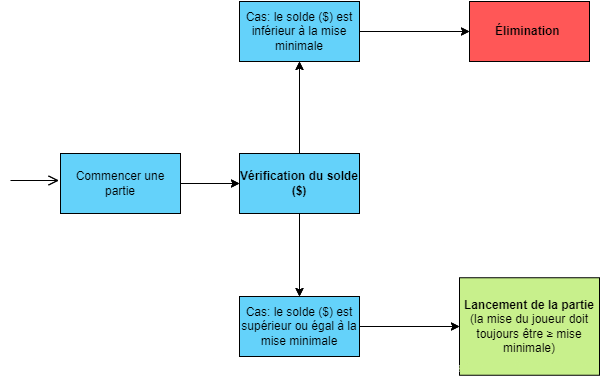
\includegraphics[width=\textwidth]{{2-besoins/diagramme_utilisation_mise_min.png}}
        \caption{Schéma d'utilisation de la mise minimale par le moteur de jeu pour l'intégration d'un joueur à une partie}
        \label{fig:diag_use_min_bet}
    \end{figure}
    
    \item \textbf{Sélectionner la mise maximum:}\\
    L'argument \code{--mise-max} détermine la mise maximum par joueur. Cet argument est optionnel. Si il n'est pas renseigné alors il n'y a pas de mise maximum (dans la limite où le joueur peut miser une telle quantité). La valeur de mise doit être comprise entre 5 et 100 000 inclus. \\
    \textbf{Priorité :} 3. \\
    \textbf{Risques :}
    \begin{itemize}
        \item une valeur inférieure à 5 est donnée.
        \item une valeur supérieure à 100 000 est donnée.
    \end{itemize}
    \textbf{Parade :} Afficher un message d'erreur, spécifiant le type d'erreur rencontré.

    \item \textbf{Afficher un récapitulatif des paramètres:} \\
    Avant l'exécution des parties, le lanceur de moteur de jeu affichera les paramètres renseignés afin que l'utilisateur puisse voir les paramètres d'exécution. \\
    \textbf{Priorité :} 3. \\
    \textbf{Risques :} aucun. \\
    \textbf{Parade :} aucune.

    \item \textbf{Lancer le programme en exécution rapide:} \\
    Lorsqu'il n'y a que des IA qui jouent, le paramètre \code{--rapide} permet de n'afficher que les résultats de chaque partie (et pas le détail de chaque tour). L'intérêt est de pouvoir exécuter beaucoup de parties rapidement et sans affichage superflu car, par exemple, nous souhaitons tester l'IA ou observer uniquement la finalité de chaque partie de Blackjack.
    Lorsque cet argument est utilisé alors qu'il y a des joueurs humains, il n'a pas d'effet et est ignoré.\\
    \textbf{Priorité :} 3. \\
    \textbf{Risques :} aucun. \\
    \textbf{Parade :} aucune.
 
    \item \textbf{Permettre d'utiliser des raccourcis d'argument:} \\ 
    Chaque argument du logiciel devra avoir une version courte. Par exemple \code{--paquets} aura comme version courte \code{-p}. \\
    \textbf{Priorité :} 3. \\
    \textbf{Risques :} aucun. \\
    \textbf{Parade :} aucune.

\end{enumerate}


\subsubsection{Le moteur de jeu}
\label{sec:engine}

\begin{enumerate}

    \item \textbf{Appliquer les règles du Blackjack:} \\
    Le moteur doit pouvoir réaliser une partie de Blackjack conformément aux règles.
    Le moteur de jeu doit vérifier que les actions faites par les joueurs (IA ou non) sont valides et qu'elles ne viennent donc pas compromettre les règles du jeu. Si le joueur a fait une erreur, le moteur lui redemande. Si au bout de 7 fois le joueur lui répond mal, le moteur élimine le joueur. \\
    \textbf{Priorité :} 1. \\
    \textbf{Risques :} aucun. \\
    \textbf{Parade :} aucune.

    \item \textbf{Afficher l'état du jeu :} \\
    Le moteur doit être capable à chaque tour ou action de joueur d'afficher l'état de jeu et ce qu'il se passe. Il affichera les cartes jouées par chaque joueur (ainsi que le total), les cartes du croupier, les mises, la quantité d'argent totale de chaque joueur, le numéro du tour, l'état du joueur (brulé, en cours, arrété), le paquet utilisé. L'affichage sera textuel et pourra être amélioré en affichage graphique si le temps l'accorde. \\
    \textbf{Priorité :} 1. \\
    \textbf{Risques :} aucun. \\
    \textbf{Parade :} aucune.

    \item \textbf{Afficher les résultats d'une partie:} \\
    A la fin d'une partie, le moteur doit pouvoir afficher le ou les gagnants, les mises gagnées et perdues par joueur, et l'état du jeu. \\
    \textbf{Priorité :} 1. \\
    \textbf{Risques :} aucun. \\
    \textbf{Parade :} aucune.

    \item \textbf{Demander la mise d'un joueur:}\\
    Dans le cas où il y a un joueur humain, le moteur doit être capable au début de chaque partie de jeu de demander la mise d'un joueur en fonction de l'état du jeu. La mise ne sera valide que si le joueur a assez d'argent dans son porte-monnaie. La mise doit être supérieure à la mise minimale spécifiée au lancement de l'application. \\
    \textbf{Priorité :} 1. \\
    \textbf{Risques :} 
    \begin{itemize}
        \item le joueur n'a pas assez d'argent.
        \item une valeur inférieure à la mise minimale est donnée.
    \end{itemize}
    \textbf{Parade :} Afficher un message d'erreur, spécifiant le type d'erreur rencontré.
    
    \item \textbf{Demander une action à un joueur}
    Le moteur doit demander au joueur de lui fournir une action en fonction de l'état du jeu et mettre à jour le jeu en fonction de la-dite action. Tant que le joueur est en jeu, le moteur doit continuer à lui demander une action et mettre à jour le jeu. Si au bout de 7 fois le joueur donne une action incorrecte, il est éliminé de la partie.\\ 
    \textbf{Priorité :} 1. \\
    \textbf{Risque :} 
    \begin{itemize}
        \item une action impossible est donnée par le joueur.
    \end{itemize}
    \textbf{Parade :} Afficher un message d'erreur, spécifiant le type d'erreur rencontré, puis redemander l'action à jouer si le nombre d'essais maximum n'est pas atteint.
    
    \item \textbf{Permettre à plusieurs joueurs de jouer dans une même partie:} \\
    Le moteur de jeu doit être capable de gérer plus d'un joueur dans une même partie.\\
    \textbf{Priorité :} 2.\\
    \textbf{Risques :} 
    \begin{itemize}
        \item le moteur ne peut gérer qu'un seul joueur contre le croupier.
        \item le moteur prend en compte trop de joueur dans la partie.
    \end{itemize}
    \textbf{Parade :} Signaler l'erreur aux développeurs.
    
    \item \textbf{Afficher les statistiques liées à un ensemble de parties :}
    \label{itm:stats}
    \\
    Les statistiques à afficher sont : la carte la plus fréquente, la carte qui gagne le plus souvent, la mise moyenne, la mise la plus petite, la mise la plus grande, les victoires par joueurs, le nombre de tour moyen. \\
    \textbf{Priorité :} 2. \\
    \textbf{Risques :} aucun. \\
    \textbf{Parade :} aucune.
    
\end{enumerate}

\subsubsection{Le joueur humain}
\label{sec:human}

Le joueur humain est le joueur assis devant l'ordinateur qui à chaque fois est interrogé par le moteur au sujet de son action à jouer pour le tour actuel. Dans ce cas, nous prenons l'exemple de l'interface textuelle. Il demandera son action via texte. Il affichera un rappel des actions possibles au blackjack ainsi que le texte à rentrer pour la faire. Si le texte entré par l'utilisateur est valide, il envoie l'action correspondante au moteur, sinon, il redemande à l'utilisateur de saisir un texte en lui expliquant l'erreur qu'il a commise (un certain nombre de fois). 
\begin{enumerate}
    \item \textbf {Miser :} \\
    Il s'agit de l'action liée à la quantité d'argent que le joueur souhaite miser en début de partie. Cette action est demandée en début de partie obligatoirement et ne peut pas être renouvelée par la suite. \\
    \textbf{Priorité :} 2 \\
    \textbf{Risque :} Le joueur entre une valeur de mise supérieure à sa quantité d'argent. \\
    \textbf{Parade :} Afficher un message d'erreur puis redemander la mise au joueur.\\
    \item \textbf {Demander une carte (piocher) :} \\
    Le texte à rentrer pour demander à piocher une carte est \code{carte}, et peut être abrégé par \code{c}. \\
    \textbf{Priorité :} 2 \\
    \textbf{Risque :} Le joueur entre une commande autre que celle spécifiée pour piocher. \\
    \textbf{Parade :} Afficher un message d'erreur puis redemander l'action au joueur.\\
    \item \textbf {Doubler sa mise :} \\
    Le texte à rentrer pour doubler sa mise est \code{double}, et peut être abrégé par \code{d}.
    Il n'est pas possible de piocher par la suite ni de faire une quelconque autre action. \\
    \textbf{Priorité :} 2 \\
    \textbf{Risque :} Le joueur demande de doubler alors qu'il n'a pas la quantité d'argent nécessaire.  \\
    \textbf{Parade :} Afficher un message d'erreur puis redemander une action.\\
    \item \textbf {Se coucher (se retirer) :} \\
    Le texte à rentrer pour se retirer de la partie en cours \code{reste}, et peut être abrégé par \code{r}. Par le biais de cette action le joueur s'arrête de jouer et récupère alors la moitié de sa mise posée au départ. \\
    \textbf{Priorité :} 2 \\
    \textbf{Risque :} Le joueur entre une commande autre que celle spécifiée pour se coucher. \\
    \textbf{Parade :} Afficher un message d'erreur puis redemander une action au joueur.\\
    \item \textbf {Abandonner :} \\
    Le texte à rentrer pour abandonner la partie est \code{abandon}, et peut être abrégé par \code{a}. \\
    \textbf{Priorité :} 2 \\
    \textbf{Risque :} Le joueur entre une commande autre que celle spécifiée pour abandonner. \\
    \textbf{Parade :} Afficher un message d'erreur puis redemander une action au joueur.\\
\end{enumerate}


\subsubsection{Le joueur Intelligence Artificielle}
\label{sec:ia}
\begin{enumerate}
    \item \textbf{Appliquer la stratégie "Basique":} \\
        Le joueur IA doit pouvoir réaliser des actions de jeu conformément aux règles et à la stratégie "Basique", qui correspond à réaliser une certaine action suivant la probabilité de tirer une carte à la valeur avantageuse (cf. \nameref{sec:basic}).
        Cette probabilité est calculée pendant le tour du joueur IA, en comptant les cartes distribuées durant la partie.\\
        \textbf{Priorité :} 1. \\
        \textbf{Risques :} aucun. \\ 
        \textbf{Parade :} aucune.

    \item \textbf{Appliquer la stratégie "Hi-Lo":} \\
        Le joueur IA doit pouvoir réaliser des actions de jeu conformément aux règles et à la stratégie "Hi-Lo", qui fait partie des stratégies les plus simples et populaires du Blackjack (cf. \nameref{sec:hilo}). 
        Elle consiste à assigner une valeur entre -1, 0 et 1 pour chaque carte dans sa main et celle des autres joueurs et du croupier. Nous avons les valeurs suivantes : -1 pour les buches, 0 pour 7, 8 et 9, puis 1 pour les autres cartes. Ainsi il est possible de facilement juger sa main et de la comparer aux autres.\\
        \textbf{Priorité :} 1. \\ 
        \textbf{Risques :} aucun. \\ 
        \textbf{Parade :} aucune.

    \item \textbf{Appliquer la stratégie "Hi-Lo No Count":} \\
        Le joueur IA doit pouvoir réaliser des actions de jeu conformément aux règles et à la stratégie "Hi-Lo No Count" (cf. \nameref{sec:hilonc}). 
        Elle consiste à assigner une valeur entre -1, 0 et 1 pour chaque carte dans sa main. Nous avons les valeurs suivantes : -1 pour les buches, 0 pour 7, 8 et 9, puis 1 pour les autres cartes. Cependant, cette version diffère de la stratégie "Hi-Lo", car elle ne compte pas les cartes apparaissant au cours de la partie.\\
        \textbf{Priorité :} 2. \\ 
        \textbf{Risques :} aucun. \\ 
        \textbf{Parade :} aucune.

    \item \textbf{Appliquer la stratégie "Deep Learning":} \\
        Le joueur IA doit pouvoir réaliser des actions de jeu conformément aux règles du blackajck et à la stratégie "Deep Learning". Celle-ci réalise une certaine action suivant la probabilité de cette dernière, d'après ce que l'IA a appris via les stratégies citées précédemment (cf. \nameref{sec:deep}). Au début de la partie, un réseau de neurones est créé puis entraîné, pour réaliser par la suite les actions qui lui semblent les plus cohérentes lors de son tour. \\
        \textbf{Priorité :} 1. \\
        \textbf{Risques :} aucun. \\ 
        \textbf{Parade :} aucune.
\end{enumerate}

\subsection{Besoins non fonctionnels}

\subsubsection{Besoins Utilisateur}
\begin{enumerate}

    \item \textbf{L'interface du logiciel doit être en français :} \\
    L'interface du programme du jeu doit être compréhensible et écrite en français courant. \\
    \textbf{Priorité :} 1. \\
    \textbf{Risques :} 
    \begin{itemize}
        \item L'affichage et l'interface ne sont pas entièrement en français. \\
    \end{itemize}
    \textbf{Parade :} Signaler l'erreur aux développeurs.
    
    \item \textbf{Le logiciel ne doit avoir accès qu’aux fichiers fournis et pas aux autres disponibles sur la machine :} \\
    \textbf{Priorité :} 1. \\
    \textbf{Risque :} 
    \begin{itemize}
        \item le logiciel accède à des fichiers auxquels il ne devrait pas.
    \end{itemize}
    \textbf{Parade :} Arrêter le chargement du fichier et arrêter le logiciel.
    
     \item \textbf{Le logiciel doit avoir une notice d'utilisation incluse :} \\
    Accessible par une option (comme \code{--help}) si le logiciel est en ligne de commande ou bien un bouton affichant cette notice dans le cas d'un logiciel ayant un affichage graphique. \\
    \textbf{Priorité :} 2. \\
    \textbf{Risques :} aucun. \\
    \textbf{Parade :} aucune.
    
    \item \textbf{Le logiciel doit avoir une version} \\
    Le paramètre \code{--version} affichera la version du logiciel.\\
    \textbf{Priorité :} 3. \\
    \textbf{Risques :} aucun. \\
    \textbf{Parade :} aucune.

\end{enumerate}

\subsubsection{Besoins Système}
\begin{enumerate}
    \item \textbf{Le logiciel doit pouvoir être éxecuté sur GNU/Linux :} \\
    \textbf{Priorité :} 1. \\
    \textbf{Risque(s) :} 
    \begin{itemize}
        \item l’OS ne permet pas d’exécuter le programme.
    \end{itemize}
    \textbf{Parade :} lister les OS et les versions exactes compatibles.
    
    \item \textbf{Le logiciel doit respecter des contraintes de performance :} \\
    \textbf{Priorité :} 1. \\
    \textbf{Risque(s) :} 
    \begin{itemize}
        \item Le lanceur de moteur de jeu doit s'exécuter en moins d'une seconde.
        \item Une IA doit répondre si possible en moins de 10 secondes.
    \end{itemize}
    \textbf{Parade :} Signaler le problème aux développeurs.
\end{enumerate}

\clearpage

\subsection{Diagramme de cas d'utilisation général}

\begin{figure}[H]
    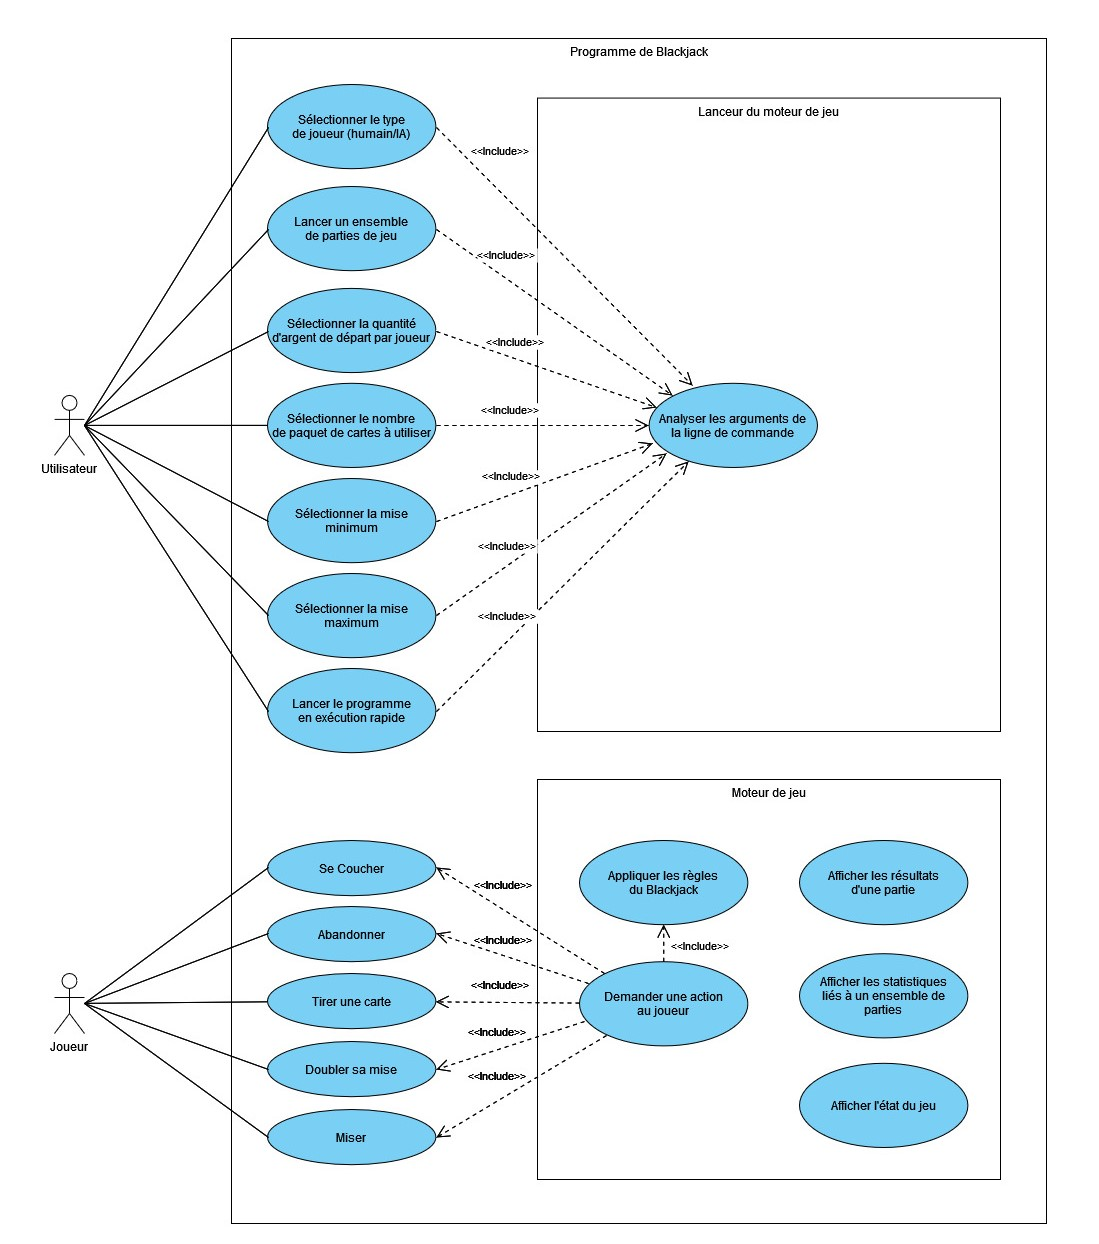
\includegraphics[width=\textwidth]{{2-besoins/diag_cas_util_general_entier.jpg}}
    \caption{Diagramme de cas d’utilisation représentant les principales interactions avec le programme}
    \label{fig:diag_use_case_general}
\end{figure}

\clearpage

\subsection{Description de l'IA}

\subsubsection{Stratégie "Basique"}
\label{sec:basic}

L'IA va déterminer la meilleure action suivant l'état de sa main en évaluant sa valeur. L'algorithme utilisé est probabiliste, c'est-à-dire qu'en fonction des cartes déjà tirées depuis le début de la partie (pour un même paquet), il calcule la probabilité pour chaque carte restante d'être tirée. Si la probabilité d'une carte ayant une valeur intéressante dépasse un certain seuil, précisé en entrée, l'algorithme choisira l'action appropriée. Par exemple, si notre main de départ à une valeur de 11, l'IA va calculer la probabilité de piocher une carte ayant une valeur entre 10 et 6. Ainsi, si cette probabilité est supérieure au seuil haut (ex: 90\%),renvoie l'action "doubler". Cependant, si elle est inférieure au seuil haut mais reste supérieure au seuil bas (ex: 70\%), la probabilité de piocher une bonne carte reste correcte, donc nous renvoyons l'action "piocher".
Ces calculs de probabilité sont effectués seulement si la valeur de la main est inférieure ou égale à une valeur arbitraire. Après une recherche empirique, nous avons estimé que cette valeur serait 17. Ainsi, si la valeur de la main est supérieure, alors l'action renvoyée est "se coucher". De ce fait, ce comportement permet d'éviter sobrement les prises de risque lorsque la main est acceptable.\\
Cet algorithme a une complexité polynomiale en O(m + d), m étant le nombre de cartes dans la main du joueur et d la taille de la collection des cartes comptées (la matrice dynamique md). \\
\\
Algorithme abstrait de la stratégie "Basique" du joueur IA :
\begin{minted}
{md}
Entrées :
main : cartes en main.
p : numéro du paquet.
sh : un seuil haut.
sb : un seuil bas.
argent : la quantité d'argent possédée.
mise : la mise effectuée.

Sortie :
Une action à jouer.

Début.
Pour chaque carte c dans main,
    Ajouter la valeur de c à somme.

Si somme est inférieure ou égale à 17 alors,
    Soustraire somme à 21 et affecter la valeur obtenue à v.

    Pour chaque carte d distribuée ce tour,
        Ajouter à une matrice dynamique md la valeur de d par rapport au paquet p.

    Pour chaque carte c du paquet,
        Si c n’appartient pas à md par rapport au paquet p alors,
            Pour i allant de 0 à 4 inclus,
                Si la valeur de c est égale à la valeur de v - i alors,
                    Incrémenter de 1 t[i].

    max prend la valeur maximum de t.

    Diviser max par la taille de md par rapport au paquet p et affecter la valeur à proba.

    Si proba est supérieure à sh alors,
        Si mise multipliée par 2 est supérieure ou égale à argent alors,
            Retourner l'action Piocher.
        Sinon, 
            Retourner l'action Doubler.
    Si proba est supérieure à sb alors,
        Retourner l'action Piocher.
             
Retourner l'action Arrêter.
Fin.
\end{minted}


\subsubsection{Stratégie "Hi-Lo"}
\label{sec:hilo}

L'IA va déterminer la meilleure action suivant l'état de sa main en évaluant sa valeur, mais également en évaluant la valeur des cartes précédemment distribuée. Cet algorithme diverge de la stratégie "Basique" de part sa manière de compter les cartes. En effet, une carte de valeur 1, 2, 3, 4, 5 ou 6 sera comptée comme une valeur de 1, une carte de valeur 7, 8 ou 9 comme un 0 et une carte de valeur 10 ou 11 comme un -1. Ainsi, en comptant les cartes distribuées avec cette technique, nous pouvons déterminer les valeurs des cartes restantes dans le paquet. Puis en fonction de la valeur de sa main, l'IA peut choisir l'action appropriée. \\
Cet algorithme a une complexité polynomiale en O(m), m étant le nombre de cartes dans la main du joueur. \\
\\
Algorithme abstrait de la stratégie "Hi-Lo" du joueur IA :
\begin{minted}
{md}
Entrées :
main : cartes en main.
p : numéro du paquet.

Sortie :
Une action à jouer.

Début.
Pour chaque carte c dans main,
    Si la valeur de c est égale à 1 ou 2 ou 3 ou 4 ou 5 ou 6 alors,
        ajouter 1 à somme.
    Si la valeur de c est égale à 10 ou 11 alors,
        ajouter -1 à somme.

Diviser somme par la taille de main et affecter la valeur obtenue à u.

Si u est supérieure à 0.5 alors,
    Retourner l'action Piocher.

Si u est inférieure à -0.5 alors,
    Retourner l'action Arrêter.

Pour chaque carte d distribuée ce tour,
    Incrémenter de 1 nombres[p].
    Si la valeur de d est égale à 1 ou 2 ou 3 ou 4 ou 5 ou 6 alors,
       ajouter 1 à sommes[p].
    Si la valeur de d est égale à 10 ou 11 alors,
       ajouter -1 à sommes[p].

Diviser sommes[p] par nombres[p] et affecter la valeur obtenue à v.

Si u est supérieure ou égale à -0.5 et inférieure à 0 et v est supérieure à 0.5, 
ou u est inférieure ou égale à 0.5 et supérieure à 0 et v est inférieure à -0.5 alors,
    Retourner l'action Doubler.

Retourner l'action Arrêter.
Fin.
\end{minted}

\subsubsection{Stratégie "Hi-Lo No Count"}
\label{sec:hilonc}

Cette stratégie se repose sur l'algorithme Hi-Lo développé précédemment. Cependant, cette version d'Hi-Lo ne compte pas les cartes apparaissant au cours de la partie. Ainsi, cette stratégie se concentre uniquement sur la manière de calculer la valeur de la main. Nous attribuons donc les nouvelles valeurs 1, 0 et -1 aux cartes. L'avantage de cette stratégie est qu'elle reste constante sur un ensemble de partie, ce qui permet alors de comparer les résultats avec la stratégie Hi-Lo basée sur le comptage des cartes. \\
Cet algorithme a une complexité polynomiale en O(m), m étant le nombre de cartes dans la main du joueur. \\
\\
Algorithme abstrait de la stratégie "Hi-Lo No Count" du joueur IA :
\begin{minted}
{md}
Entrées :
main : cartes en main.

Sortie :
Une action à jouer.

Début.
Pour chaque carte c dans main,
    Si la valeur de c est égale à 1 ou 2 ou 3 ou 4 ou 5 ou 6 alors,
       ajouter 1 à somme.
    Si la valeur de c est égale à 10 ou 11 alors,
       ajouter -1 à somme.

Diviser somme par la taille de main et affecter la valeur obtenue à u.

Si u est supérieure à 0.5 alors,
    Retourner l'action Piocher.

Retourner l'action Arrêter.
Fin.
\end{minted}

\subsubsection{Algorithme de mise des stratégies "Basique" et "Hi-Lo"}

Cet algorithme de mise est basé sur le comptage de carte et est donc partagé par les stratégies "Basique" et "Hi-Lo". Puisque ces stratégies sont de plus en plus performantes lorsque de plus en plus de cartes sont comptées, les mises effectuées par l'IA se base sur le nombre de cartes comptées. Sur un ensemble de partie, les mises réalisées seront donc progressivement plus importantes. L'algorithme se base également sur la somme actuelle d'argent possédée par l'IA. Cela permet de garantir que l'IA misera une somme en accord avec ce qu'elle possède et donc éviter des mises impossibles. \\
Cet algorithme a une complexité polynomiale en O(1). \\
\\
Algorithme abstrait de mise des joueurs IA "Basique" et "Hi-Lo" :
\begin{minted}
{md}
Entrées :
p : numéro du paquet.
argent : la quantité d'argent possédée.
misemin : mise minimale acceptée.
misemax : mise maximale acceptée.

Sortie :
Une valeur à miser.

Début.
mise prend la valeur misemin.

Si le nombre de cartes comptées pour le paquet p est supérieur à 0 alors,
    Multiplier argent par le nombre de carte comptée et affecter la valeur obtenue à m.
    Diviser m par la taille d'un paquet complet et affecter la valeur obtenue à mise.
    
    Si mise est inférieure à misemin alors,
        mise prend la valeur misemin.
        
    Si mise est supérieure à misemax alors,
        mise prend la valeur misemax.

Retourner mise.
Fin.
\end{minted}

\subsubsection{Stratégie Deep Learning}
\label{sec:deep}

\paragraph{Explication générale}
Cette intelligence artificielle est fortement basée sur les stratégies "Basique" et "Hi-Lo". En effet, comme son nom l'indique, elle s'appuie sur un réseau de neurones artificiel, qui permettent à l'IA d'apprendre. Pour se faire, il faut ce que nous appelons un ensemble de données (dataset) à fournir à notre réseau. Nous avons crée nos propres données regroupées sous la forme d'un fichier CSV. Ce fichier CSV contient donc un ensemble de partie, et pour chacune d'entre elles, nous savons quel type d'IA a joué, si elle a gagné, les cartes qu'elle avait, ainsi que les cartes que possédait le croupier. Ci-dessous, un extrait du format du fichier qui est utilisé. \\

\begin{figure}[H]
    \csvautotabular{2-besoins/dataset_exemple.csv} 
    \caption{Extrait du fichier CSV utilisé pour créer le dataset}
    \label{fig:csv_exemple}
\end{figure}

Cependant, le fichier n'est pas utilisé tel quel. Il faut formater les données, mais aussi choisir uniquement les informations que nous considérons essentielles au bon fonctionnement du réseau de neurones, et un temps de calcul raisonnable. Pour cela, nous considérons uniquement deux dimensions, qui sont la somme des cartes du joueur (ici c'est une IA développée précédemment), ainsi que la première carte du croupier car au moment de la partie, nous ne connaissons qu'une seule carte du croupier, celle face visible. Nous avons donc en entrée un vecteur de taille 2, qui va être traité par le réseau de neurones, et en sortie nous avons un vecteur de taille 4. Chaque élément de ce vecteur de sortie est exprimé sous la forme d'une probabilité et se réfère donc à une action possible lors de la partie. Le premier élément correspond à l'action de piocher, le second à l'action de rester, le troisième à l'action de doubler et enfin le dernier à l'action d'abandonner. Lors d'une partie, l'IA basée sur le deeplearning est capable de retourner l'action avec la plus haute probabilité selon ce qu'elle a appris, dans notre cas, via le fichier CSV construit au cours des parties. 

\paragraph{Réseau de neurones}
Notre réseau de neurones est constitué d'une couche d'aplatissement en entrée, de 3 couches cachées intermédiaires, et d'une couche de sortie dite softmax, qui permet d'attribuer une probabilité à chaque action selon le vecteur en entrée. 
Les trois couches cachées sont toutes de types dense, la première comporte 128 neurones, la seconde 64 et la troisième 32. Chaque couche a pour fonction d'activation la fonction ReLU qui choisi le maximum entre x (la valeur fournie) et 0. Cette fonction a été choisie car nous avons ici une classification non-binaire (plusieurs actions possibles à la fin et non uniquement deux), mais aussi car c'est une des fonctions les plus performantes et utilisées pour les couches denses dans de tels réseaux de neurones. \\
Pour la couche de sortie, il s'agit d'une couche dense de taille 4 (représentant le nombre de classes, soit le nombre d'actions possibles lors d'une partie), utilisant la fonction d'activation softmax. Comme précisé auparavant, cette couche permet de transformer notre vecteur d'entiers, en vecteurs de probabilités. C'est la fonction que nous avons choisi car elle est parfaitement adaptée aux problèmes multi-classes, comme c'est le cas ici. Nous avons ainsi une probabilité pour chaque action. 
\begin{figure}[H]
    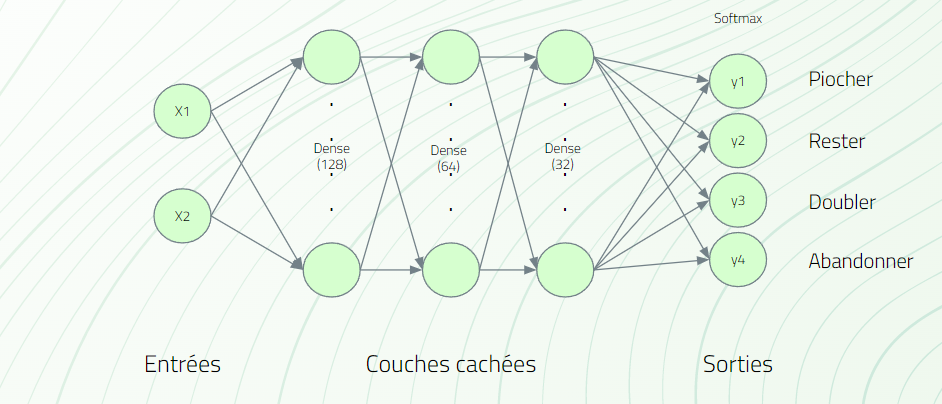
\includegraphics[width=\textwidth]{{2-besoins/reseau_neurones.png}}
    \caption{Schéma du réseau de neurones implémenté}
    \label{fig:reseau_neurones}
\end{figure} 

Enfin, lors de la compilation du modèle, il est important de choisir la bonne fonction de perte. Dans notre cas, la meilleure fonction minimisant la perte est celle calculant la moyenne des carrés des erreurs entre la vérité terrain et la prédiction. Ensuite, lors de l'entraînement du modèle, la taille des "batchs" ainsi que le nombre "d'épochs" est important. Nous avons choisi un nombre d'épochs de 256, car il faut que celui-ci soit suffisamment important lorsque la taille du dataset est considérable, ce qui est le cas. Néanmoins, il ne doit pas non plus être trop grand pour éviter le phénomène d'overfitting, ce qui pousserait notre modèle à trop se coller au set d'entraînement et donc de fournir des prédictions plutôt mauvaises. 
Pour le nombre de batchs, 64 suffit amplement, sans être trop important, également pour suivre le même raisonnement que donné juste avant. Enfin notre dataset est quant à lui partagé en deux, une partie pour l'entraînement et une partie pour tester le modèle. Nous avons choisi de donner 85\% pour l'entraînement et le reste pour les tests. Avec l'ensemble de ces paramètres nous avons un modèle avec un taux de précision aux alentours de 72\% et une perte autour de 0.1 (varie entre 0.09 et 0.1).  
\begin{figure}[H]
    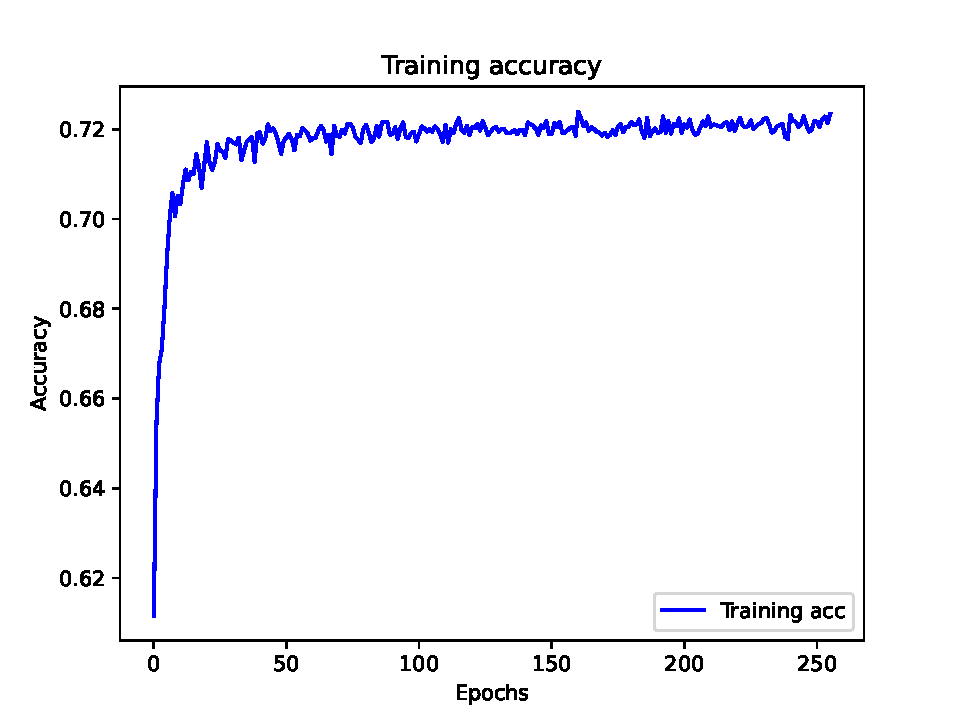
\includegraphics[width=\textwidth]{{2-besoins/acc_plot.pdf}}
    \caption{Précision du modèle au cours de l'apprentissage}
    \label{fig:plot_acc_modele}
\end{figure} 

\begin{figure}[H]
    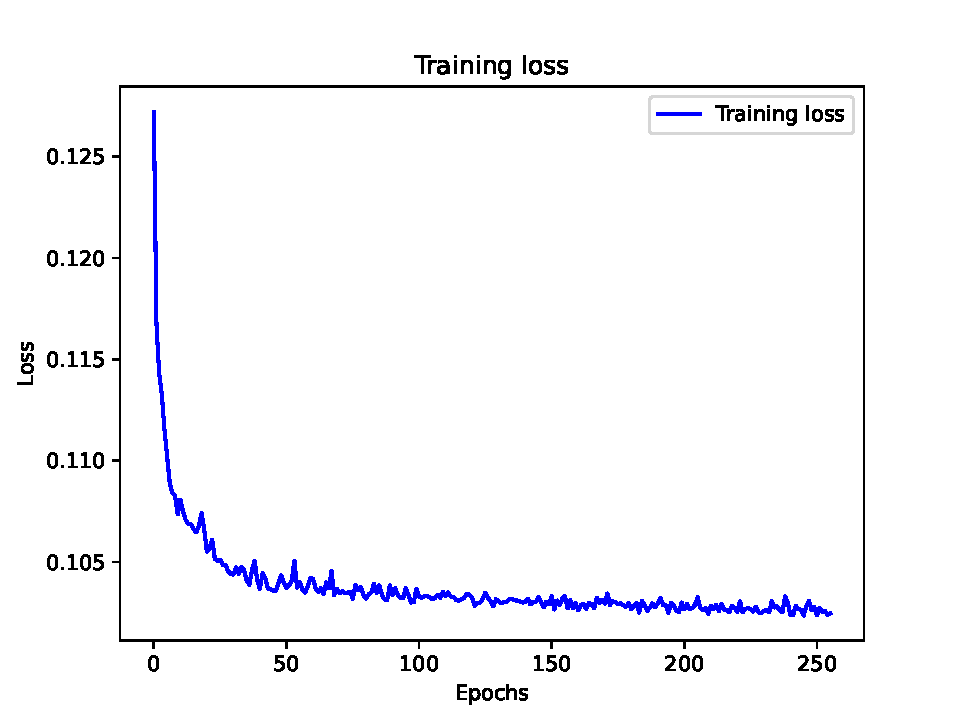
\includegraphics[width=\textwidth]{{2-besoins/loss_plot.pdf}}
    \caption{Fonction de perte du modèle au cours de l'apprentissage}
    \label{fig:plot_loss_modele}
\end{figure} 

\paragraph{Recherches des paramètres}

Afin d'atteindre de tels résultats, il a fallu passer par des périodes de recherches pour trouver des bons paramètres. Au départ, notre vecteur en entrée était de taille 6, puis nous avons vu que certains critères n'influençaient pas sur la prédiction, donc les retirer était plus pertinent. Ensuite, la répartition des données entre apprentissage et test était respectivement de 70\% et 30\%, donc nous avons favorisé l'apprentissage en donnant 85\% des données. Une légère augmentation de la précision du modèle a pu être observée via la modification de ces deux paramètres (de 65\% à 69\%). \\
Nous nous sommes alors dirigés ensuite sur le nombre de couches cachées et leurs tailles. En ajouter ne procurait aucune amélioration de la précision. Quant à la taille des épochs et des batchs, les augmenter a permis d'avoir une meilleure précision (autour de 70\%), mais la perte pendant ce temps restait toujours très élevée (environ 0.8). Il a fallu simplement changer la fonction de perte qui était de base "cross entropy" en "mean squared error". Nous avons eu une descente de la perte aux alentours de 0.1. La cross entropy pouvait sembler correspondre, or le problème est qu'elle ne sert qu'à calculer des différences entre des probabilités. Pour notre vérité terrain, une probabilité est au maximum et les autres à zéro ce qui augmente la perte. C'est pourquoi la moyenne des carrés des erreurs est plus favorable dans notre cas, avec l'utilisation de probabilités comme nous l'avons fait pour la vérité terrain et les prédictions. 
